\chapter{Swift}

\section{Cenni storici}
Lo sviluppo di Swift è iniziato nel 2010 da Chris Lattner, aiutato in seguito da molti altri programmatori. Swift ha preso idee "da Objective-C, Rust, Haskell, Ruby, Python, C\#, CLU, e molti altri".Il 2 giugno 2014 l'app per il WWDC è divenuta la prima app distribuita al pubblico scritta in Swift.\\Il 3 dicembre 2015 viene lanciato il sito swift.org ed il codice sorgente del linguaggio è pubblicato con licenza Apache 2.0 sul repository GitHub dell'azienda.\\Apple resta lo sviluppatore principale e ne rende disponibile anche una versione del compilatore per Linux (Creato appositamente per Ubuntu).\\Il 13 settembre 2016, durante la WWDC 2016, Apple ha presentato la terza versione del suo linguaggio di programmazione insieme ad un'applicazione per iPad, Swift Playgrounds, che permette, tramite una grafica semplice e intuitiva, di imparare a programmare con Swift, soprattutto orientato ai più giovani.
\section{Caratteristiche}
\subsection{Sintassi}
\subsubsection{Implementazione di una classe}
In Swift, al contrario di molti altri linguaggi, non ci sono 2 file distinti per l'interfaccia e l'implementazione, ma uno solo con l'estensione .swift\\
Esempio di creazione di una nuova classe:\\
\lstset{language=[Objective]C, breakindent=40pt, breaklines}
\begin{lstlisting}
class Persona { 

//dichiarazione delle properties

	var nome: String? 
	var cognome: String? 
	var eta: Int?

//costruttore personalizzato con parametri 

	init(nome: String, cognome: String, eta: Int) {
		self.nome = nome
		self.cognome = cognome
		self.eta = eta
	}

//dichiarazione dei metodi setter e getter 

	func getNome() -> String {

		return self.nome
	}

	func setNome(nome: String) {

		self.nome = nome
	}

	func getCognome() -> String {

		return self.cognome
	}

	func setCognome(cognome: String) {
	
		self.cognome = cognome
	}

	func getEta() -> Int {
	
		return eta
	}

	func setEta(eta: Int) {

		self.eta = eta
	}
}
\end{lstlisting}
\subsubsection{Dichiarazione e definizione dei metodi}
In Swift, una dichiarazione di funzione (metodo) ha la seguente sintassi: 
\lstset{language=[Objective]C, breakindent=40pt, breaklines}
\begin{lstlisting}
//Nell'ordine: func nomeMetodo(nomeArg1:tipoArg1) -> tipoDiRitorno

func calcolaEta(dataDiNascita: NSDate) -> Int

\end{lstlisting}
Definizione del metodo appena dichiarato: 
\lstset{language=[Objective]C, breakindent=40pt, breaklines}
\begin{lstlisting}
func calcolaEta(dataDiNascita: NSDate) -> Int

	let oggi = Date()
      
    let componentiCalendario = Calendar.current.dateComponents([.year], from: dataDiNascita, to: oggi)                             			
	
	let eta = componentiCalendario.year!
	
	return eta;
}
\end{lstlisting}
Le funzioni in Swift sono trattate come oggetti, ciò significa che una funzione può ritornare un'altra funzione: 
\lstset{language=[Objective]C, breakindent=40pt, breaklines}
\begin{lstlisting}
func creaIncrementatore() -> ((Int) -> Int) {
	
	func aggiungiUno(numero: Int) -> Int {
	
		return 1 + numero 
	
	}
	
	return aggiungiUno
}

var incrementatore = creaIncrementatore()
incrementatore(7)
\end{lstlisting}
\subsubsection{Closures}
Le funzioni sono un caso speciale di "closure": il codice in una closure ha accesso a variabili e funzioni che sono disponibili nel suo scope, anche se viene eseguita in uno scope diverso. Una closure viene definita dalla sintassi \{ \}, utilizzando il separatore \"in\" per gli argomenti e il tipo di ritorno dal corpo:\\\\ 
\lstset{language=[Objective]C, breakindent=40pt, breaklines}
\begin{lstlisting}
var numeri = [2,25,21,89,90]

numeri.map({
	(numero: Int) -> Int in 
	let risultato = 3 * numero 
	return risultato 
})
\end{lstlisting}
Ci sono vari modi per scrivere le closure: quando il tipo è già conosciuto, come per esempio in una callback per un delegate, si possono omettere i tipi dei parametri, il tipo di ritorno o entrambi nel caso in cui ci sia un singolo statement, in quanto la closure ritorna implicitamente il valore di ritorno:
\lstset{language=[Objective]C, breakindent=40pt, breaklines}
\begin{lstlisting}
let numeriInMap = numeri.map({ numero in 3 * numero })
\end{lstlisting}
Ci si può riferire ai parametri per numero invece che per nome, approccio utile specialmente in closure che richiedono poco codice; una closure passata come ultimo argomento di una funzione può essere scritta immediatamente dopo le parentesi, e se quest'ultima è l'unico argomento della funzione stessa si possono omettere le parentesi tonde: 
\lstset{language=[Objective]C, breakindent=40pt, breaklines}
\begin{lstlisting}
//ordino i numeri in modo crescente

let numeriOrdinati = numeri.sorted { $0 > $1 }
\end{lstlisting}
\subsubsection{Enumerazioni}
La sintassi enum è utilizzata per dichiarare le enumerazioni in Swift. La particolarità rispetto ad Objective-C è che quest'ultime possono contenere metodi:
\lstset{language=[Objective]C, breakindent=40pt, breaklines}
\begin{lstlisting}
enum TipologieDiCase {

	case condominio, villa, indipendente, attico
	
	func descrizione() -> String {
	
		switch self {
	
		case .condominio:
			return "Condominio"
		case .villa :
			return "Villa"
		case .indipendente:
			return "Casa indipendente"
		case .attico
			return "Attico"
		default: 
			return String(self.rawValue)
		
		}
	}
}

let villa = TipologieDiCase.villa
let descrizioneVilla = villa.descrizione()
\end{lstlisting}
\subsubsection{Protocolli ed estensioni}
Un protocollo definisce un'interfaccia di metodi, variabili ed altri eventuali requisiti che definiscono una particolare funzionalità. Quest'ultimo può essere quindi adottato da una classe, struct o enum che ne forniranno l'implementazione:
\lstset{language=[Objective]C, breakindent=40pt, breaklines}
\begin{lstlisting}
protocol ProtocolloDiNavigazioni {
	
	func navigaAlleImpostazioni(sender: CollectionView) 
	func navigaAlDettaglioEvento(sender: UICollectionView)
}

class MenuPrincipale: UICollectionViewController, UICollectionViewDelegateFlowLayout: ProtocolloDiNavigazioni {

	override func viewDidLoad() {
        super.viewDidLoad()
		collectionView?.delegate = self
		collectionView?.dataSource = self
	}
	
	...
	
	//MARK: CollectionViewDelegate 
	
	override func collectionView(collectionView: UICollectionView, didSelectItemAtIndexPath indexPath: NSIndexPath) {
		
		switch indexPath {
			
			case 0: 
				navigaAlleImpostazioni(self.collectionView)
			case 1:
				navigaAlDettaglioEvento(self.collectionView)
		}
	}	
		
	//MARK: Implementazione del protocollo 
		
	func navigaAlleImpostazioni(sender: UICollectionView) {
        
        appDelegate.gotoSettingsVC()
    }
    
    func navigaAlDettaglioEvento(sender: UICollectionView) {
        
        appDelegate.gotoEventDetailVC()
    }
}
\end{lstlisting}
Le estensioni sono invece un modo per aggiungere funzionalità ad un tipo eisstente, come nuovi metodi e computed properties:
\lstset{language=[Objective]C, breakindent=40pt, breaklines}
\begin{lstlisting}
//Estensione che aggiunge un effetto di blur ad una imageView

extension UIImageView
{
    func aggiungiBlur()
    {
        let blurEffect = UIBlurEffect(style: UIBlurEffectStyle.Light)
        let blurEffectView = UIVisualEffectView(effect: blurEffect)
        blurEffectView.frame = self.bounds
        self.addSubview(blurEffectView)
    }
}

let containerImmagine = UIImageView()
containerImmagine.image = UIImage(named: "beer2beerlogo.jpg")
containerImmagine.aggiungiBlur()
\end{lstlisting}
\subsubsection{Gestione degli errori}
Gli errori vengono rappresentati utilizzando qualsiasi tipo che si conformi al protocollo Error; la parola chiave throws viene utilizzata per indicare che una funzione può ritornare un errore, utilizzando la parola chiave throw. Se si lancia un errore dall'interno di una funzione, quest'ultima ritorna immediatamente e l'errore viene gestito dalla funzione chiamante:
\lstset{language=[Objective]C, breakindent=40pt, breaklines}
\begin{lstlisting}
enum ErroriStampante: Error {

	case cartaEsaurita
	case inchiostroEsaurito
	case cassettoChiuso
	
}

func invia(lavoro: Int, allaStampante nomeStampante: Stringa) throws -> String {
	if nomeStampante = "Rusty old printer" {
		
		throw ErroriStampante.cassettoChiuso
	}

	return "Lavoro inviato alla stampante"
}

	do {
	
	let rispostaStampante = try invia(lavoro: 2303, allaStampante: "Sala meeting")
	
	print(rispostaStampante)
	
	} catch {
		
		print(error)
	}
	
\end{lstlisting}
Si possono inoltre utilizzare più blocchi catch per gestire errori specifici:
\lstset{language=[Objective]C, breakindent=40pt, breaklines}
\begin{lstlisting}
	do {
	
		let rispostaStampante = try invia(lavoro: 2303, allaStampante: "Sala 	meeting")
	
		print(rispostaStampante)
	
		} catch ErroriStampante.cassettoChiuso {
		
			print("Aprire il cassetto")
		}
\end{lstlisting}
Un altro modo per gestire gli errori è quello di utilizzare la parola chiave try? per convertire il risultato in un tipo optional: se la funzione lancia un errore, questo specifico errore è ignorato e la funzione ritorna nil; alternativamente il risultato è un optional contenente il valore ritornato dalla funzione:
\lstset{language=[Objective]C, breakindent=40pt, breaklines}
\begin{lstlisting}
let foglioStampato = try? invia(lavoro: 1984, allaStampante: "Sala meeting")
let erroreDiStampa = try? invia(lavoro: 1948, allaStampante: "Rusty old printer")
\end{lstlisting}
\subsubsection{Generics}
Una funzione generica, più comunemente chiamata template, è così dichiarata:
\lstset{language=[Objective]C, breakindent=40pt, breaklines} 
\begin{lstlisting}
func creaArray<Elemento>(ripeti	elemento: Elemento, numeroDiVolte: Int) -> [Elemento] {

	var risultato = [Elemento]()
	
	for _ in 0..< numeroDiVolte {
		
		risultato.append(elemento)
	}
	
	return risultato
}

//chiamata alla funzione 

creaArray(ripeti: "Tick tock", numeroDiVolte: 3)
\end{lstlisting}
Si possono creare generics di funzioni o di classi, enumerazioni e struct:
\lstset{language=[Objective]C, breakindent=40pt, breaklines}
\begin{lstlisting}
//Reimplementazione del tipo optional della libreria standard di Swift

enum OptionalValue<Wrapped> {

	case none 
	case some(Wrapped)
}

var possibileIntero: OptionalValue<Int> = .none
possibileIntero = .some(100)
\end{lstlisting}
Si utilizza la parola chiave where prima del corpo per indicare una lista di requisiti, per esempio per indicare che il tipo deve conformarsi ad un protocol, per richiedere che due tipi siano uguali o per indicare che una classe deve avere una particolare superclasse: 
\lstset{language=[Objective]C, breakindent=40pt, breaklines}
\begin{lstlisting}
func elementiComuni<T: Sequence, U: Sequence>(_ lhs: T, _ rhs: U) -> Bool {
	
	where T.Iterator.Element: Equatable,
		  T.Iterator.Element == U.Iterator.Element {
		  
		  	for lhsItem in lhs {
		  	
		  		for rhsItem in rhs {
		  		
		  			if lhsItem == rhsItem {
		  				
		  				return true
		  			}
		  		}
		  	}
		  }
		  
		  return false
}

//chiamata alla funzione 

elementiComuni([1,2,3], [3])
\end{lstlisting}
\subsubsection{Tuples}
Feature non presente in Objective-C, le tuple raggruppano più valori (di un tipo qualsiasi o tipi differenti) in un singolo valore composto. Per esempio, potremmo descrivere lo status code 404 dell'HTTP con una tupla in questo modo:
\lstset{language=[Objective]C, breakindent=40pt, breaklines}
\begin{lstlisting}
let errore404http = (404, "Not found")
\end{lstlisting}
La tupla (404, "Not found") raggruppa insieme un tipo Int e uno String; si può creare qualsiasi permutazione di tipi. Per ottenere i singoli valori da una tupla, quest'ultima deve essere scomposta:
\lstset{language=[Objective]C, breakindent=40pt, breaklines}
\begin{lstlisting}
let (statusCode, statusMessage) = errore404http
\end{lstlisting}
Questo particolare tipo è utile come valore di ritorno dalle funzioni, per esempio una funzione che ha il compito di caricare una pagina web potrebbe usare la tupla sopra descritta per indicare il successo o il fallimento del caricamento, fornendo più informazioni rispetto ad un valore di ritorno singolo di un singolo tipo. 
\subsubsection{Optionals}
Questo tipo è un pilastro portante di Swift, in quanto viene utilizzato  in tutti i casi in cui il valore di ritorno potrebbe essere nullo (nil). La logica di funzionamento è la seguente: o c'è un tipo di ritorno, e quindi si utilizza l'unwrapping per accedere al valore, o non c'è valore alcuno.\\
Il concetto di optional non esiste in C o Objective-C. Ciò che ci si avvicina di più è l'abilità di ritornare nil da un metodo che altrimenti ritornerebbe un oggetto, con nil a significare l'assenza di un oggetto valido.\\Questo però funziona solamente per gli oggetti (non structs, tipi C  o enumerativi); per questi i metodi Objective-C ritornano solamente un valore speciale (come per esempio NSNotFound). Questo implica che il chiamante dei metodi sappia che c'è uno speciale valore da verificare, l'approccio di Swift permette invece di indicare l'assenza di qualsiasi valore in assoluto, senza la necessità per speciali costanti.\\
In questo esempio vediamo come gli optional possono essere utilizzati per gestire il caso di assenza di valore. Il tipo Int di Swift ha un costruttore che prova a convertire una String  in un valore di tipo Int; questa conversione può fallire e quindi viene utilizzato un tipo optional:
\lstset{language=[Objective]C, breakindent=40pt, breaklines}
\begin{lstlisting}
let possibileNumero = "123"
let numeroConvertito = Int(possibileNumero)
//numeroConvertito e' di tipo Int?, che si legge come "optional Int"
\end{lstlisting} 
Poichè il costruttore può fallire, questi ritorna un tipo optional Int, scritto Int?. Il punto di domanda indica che il valore contiene un tipo optional, il che significa che potrebbe contenere un valore Int, o nessun valore.\\
Utilizzando la speciale parola chiave nil, si indica che un tipo optional non ha valore alcuno. nil non può essere utilizzato con constanti e variabili non optional.
\lstset{language=[Objective]C, breakindent=40pt, breaklines}
\begin{lstlisting}
var codiceRispostaServer: Int? = nil
\end{lstlisting}
Se si crea una variabile optional, alla quale non si assegna alcun valore, a quest'ultima viene automaticamente assegnato nil.\\Il nil di Swift non è però equivalente a quello di Objective-C: in quest ultimo, nil è un puntatore ad un oggetto che non esiste, in Swift non è invece un puntatore, è l'assenza di valore alcuno. Optionals di qualunque tipo possono essere settati a nil, non solamente oggetti.\\
Per verificare la presenza di valore in un tipo optional è possibile usare lo statement if in questo modo: 
\lstset{language=[Objective]C, breakindent=40pt, breaklines}
\begin{lstlisting}
if numeroConvertito != nil {

	//numero convertito contiene un valore
}
\end{lstlisting}
Alternativamente è possibile utilizzare il simbolo !, letto come \"forced unwrapping\"  del tipo optional; questo approccio è rischioso e porta spesso ad errori in runtime.
Viene utilizzata molto più frequentemente la sintassi dell'optional binding, per verificare se una certa variabile optional contiene un valore e, se presente, assegnarlo ad una costante o variabile temporanea. Si utilizza con gli statement if e while:
\begin{lstlisting}
if let numero = Int(possibileNumero) {
	//se entro nel blocco significa che possibileNumero 
	//contiene un intero poiche' la conversione ad Int va a buon fine
} else {
	//possibileNumero non e' stato convertito ad Int
}
\end{lstlisting}
Questo codice può essere letto come: se l'optional Int ritornato da Int(possibileNumero) contiene un valore, assegna alla nuova costante chiamata numero il valore contenuto nell'optional. Questa costante è già stata inizializzata con il valore contenuto all'interno dell'optional, quindi non è necessario utilizzare la sintassi ! per forzare l'accesso al valore. In uno statement si possono concatenare più optional binding separati da virgola, se almeno uno di questi valori è nil o una condizione booleana valuta a false, l'intera condizione dello statement viene considerata falsa.\\
Le costanti e le variabili create tramite l'optional binding in uno statement if sono accessibili solamente all'interno dello statement stesso; per permettere l'accesso anche alle linee di codice che seguono lo statement, è necessario utilizzare lo statement guard. 
\subsection{Compilatore e libreria standard}
\subsubsection{Architettura del compilatore}
Il compilatore di Swift è composto dai seguenti componenti principali:
\begin{itemize}
\item Parser: il parser è un semplice parser ricorsivo discendente con un lexer codificato a mano. Il parser è il responsabile della generazione dell'albero di sintassi astratta senza alcuna informazione semantica o di tipo, e genera errori in caso di problemi grammaticali nel sorgente.
\item Analizzatore semantico: trasforma l'albero generato dal parser in un albero ben formato e con controllo sui tipi. Questo analisi include la type inference e in caso di successo, indica che è sicuro generare il codice dall'albero creato
\item Clang importer: Importa i moduli di Clang e mappa le API C o Objective-C nelle rispettive API Swift. Gli alberi risultanti vengono utilizzati dall'analizzatore semantico.
\item Generatore SIL: SIL è l'acronimo di Swift Intermediate Language, ovvero un linguaggio intermedio di alto livello, specifico per l'analisi e l'ottimizzazione del codice. Questa fase trasforma l'albero di sintassi astratta creato dall'analizzatore in un cosiddetto SIL "grezzo".
\item Trasformazioni SIL: Questo strumento esegue ulteriori diagnostiche che influenzano la correttezza del programma (come ad esempio l'uso di variabili non inizializzate). Il risultato finale di queste trasformazioni è SIL "canonico".
\item Ottimizzazioni SIL: Questa fase esegue ulteriori ottimizzazioni specifiche di alto livello, quali Automatic Reference Counting per la gestione della memoria, devirtualizzazione e specializzazione dei tipi generics.
\item Generazione IR LLVM: IR significa Intermediate Representation. Questa fase passa dal SIL al LLVM IR, e a questo punto LLVM può continuare ad ottimizare il codice e generare il codice macchina.
\end{itemize}
\subsubsection{Libreria standard Swift}
La libreria standard Swift comprende un certo numero di tipi di dati, protocolli e funzioni, compresi i tipi fondamentali (ad esempio, int, double), collezioni (per esempio, Array, dizionario) insieme ai protocolli che li descrivono e gli algoritmi che operano su di essi, i caratteri e stringhe, e le primitive di basso livello (ad esempio, UnsafeMutablePointer).\\
Il repository della libreria standard viene ulteriormente suddiviso:
\begin{itemize}
\item Nucleo principale: include la definizione di tutti i tipi, protocolli e funzioni.
\item Runtime: Il runtime di supporto è il componente che risiede nel mezzo tra il compilatore e il nucleo della libreria standard. E' il responsabile dell'implementazione delle features dinamiche del linguaggio, come il casting  (ad esempio per gli operatori as! ed as?) o i metadata dei tipi (per supportare i generics e la reflection) e la gestione della memoria (allocazione degli oggetti, reference counting). Differentemente dalle altre librerie di alto livello, il runtime è scritto quasi esclusivamente in linguaggio C++ o Objective-C.
\item Overlays per SDK: componenti specifici per le piattaforme Apple, forniscono modifiche ed aggiunte specifiche per Swift ai framework Objective-C, per migliorare la loro interoperabilità. 
\end{itemize}
\subsubsection{Whole module optimization}
Con la versione 3.0 di Swift è stata introdotta una modalità di ottimizzazione del compilatore che, dipendentemente dal progetto, permette miglioramenti delle performance significativi.\\
Funzionamento del compilatore senza WMO:
Un modulo è un set di files Swift, ed ogni modulo viene compilato in una singola unità di distribuzione (un framework o un eseguibile). Nella compilazione a file singolo il compilatore è invocato separatamente per ogni file nel modulo: 
\begin{figure}[H]
      \centering
      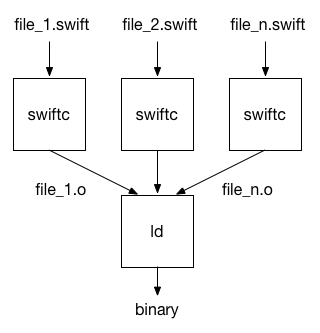
\includegraphics[scale=0.80]{immagini/single-file.png}
            \vspace{0.8cm}
            \caption{\textit{Visualizzazione del lavoro del compilatore in modalità di compilazione per ogni singolo file}}
    \end{figure}
Dopo la lettura ed il parsing del singolo file, il compilatore ottimizza il codice, genera il codice macchina e scrive un file oggetto. Successivamente il linker unisce tutti i file oggetto e genera la libreria condivisa o l'eseguibile.\\
Questa compilazione singola limita le ottimizzazione inter funzione, come l'inlining o la specializzazione dei generics alle le funzioni chiamate all'interno dello stesso file. Come esempio, assumiamo che un file di un modulo, chiamato utils.swift, contenga una struttura dati generica chiamata Container<T>, con un metodo chiamato getElement. Questo metodo è chiamato nel modulo, ad esempio nel file main.swift:
\begin{lstlisting}
//main.swift:

func add (c1: Container<Int>, c2: Container<Int>) -> Int {
  return c1.getElement() + c2.getElement()
}
\end{lstlisting}
\begin{lstlisting}
//utils.swift:

struct Container<T> {
  var element: T

  func getElement() -> T {
    return element
  }
}
\end{lstlisting}
Quando il compilatore ottimizza il file main.swift non conosce come la funzione getElement sia implementata, conosce solo il fatto che è presente; viene quindi generata una chiamata al suddetto metodo.\\
Analogamente, quando il compilatore ottimizza il file utils.swift non conosce per quale tipo concreto il metodo viene chiamato, quindi può generare solamente una versione generica della funzione, rendendo il codice più lento rispetto ad uno ottimizzato per un tipo concreto.\\
Anche solamente uno statement return in getElement necessita di un lookup di tipo per verificare come copiare l'elemento; può trattarsi di un tipo Int o di un tipo più dispendioso in termini di risorse che richiede operazioni di reference counting.
Funzionamento del compilatore con WMO:\\
Con l'ottimizzazione per l'intero modulo il compilatore ottimizza tutti i file di un modulo nella loro interezza: 
\begin{figure}[H]
      \centering
      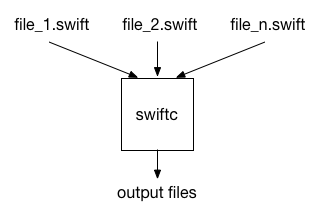
\includegraphics[scale=0.80]{immagini/wmo.png}
            \vspace{0.8cm}
            \caption{\textit{Visualizzazione del lavoro del compilatore in modalità di compilazione whole module optimization}}
\end{figure}
Questo porta due notevoli vantaggi: il compilatore vede le implementazioni di tutte le funzioni del modulo, e può quindi procedere con le ottimizzazioni specifiche; specializzare una funzione significa che il compilatore crea una nuova versione del metodo specifica per il contesto della chiamata. Ad esempio, il compilatore può ottimizzare le funzioni di tipo generics per i tipi concreti.\\
Nell'esempio, il compilatore crea una versione della struct Container specifica per i tipi Int: 
\begin{lstlisting}
struct Container {
  var element: Int

  func getElement() -> Int {
    return element
  }
}
\end{lstlisting}
Può quindi procedere all'inlining del metodo specializzato getElement all'interno della funzione add:
\begin{lstlisting}
func add (c1: Container<Int>, c2: Container<Int>) -> Int {
  return c1.element + c2.element
}
\end{lstlisting}
Contrariamente alla compilazione a file singolo, il lavoro viene eseguito in poche istruzioni macchina. La specializzazione di funzioni e l'inlining tra più file sono solo esempi delle otimizzazioni che il compilatore può apportare con l'approccio WMO, un altro campo in cui può migliorare le performance è nella gestione della memoria, in quanto il compilatore può rimuovere operazioni di reference counting ridondanti. Un altro beneficio è che il compilatore può valutare tutti gli usi di funzioni non pubbliche, con questa informazione può eliminare le cosiddette funzioni inutilizzate, ovvero quelle che non vengono mai chiamate ed usate. Potrebbe essere fuorviante il fatto che non vengano mai chiamate e quindi ci si può domandare perchè un programmatore debba scrivere una funzione che non viene mai chiamata, la ragione sta nel fatto che alcune funzioni possono diventare inutilizzate come side-effect derivante dalle altre ottimizzazioni. Riprendendo l'esempio, possiamo assumere che  la funzione add sia l'unica ad utilizzare Container.getElement. Dopo aver effettuato l'inlining della funzione getElement, la funzione non viene più utilizzata e può quindi essere rimossa. Anche se il compilatore decide di non fare l'inline della funzione, può comunque rimuovere la versione generica di getElement, poichè la funzione add utilizza solamente la versione specializzata.
\subsubsection{Tempo di compilazione}
Con l'ottimizzazione a file singolo il driver del compilatore inizia la compilazione epr ogni file in un processo separato, processo che può essere eseguito in parallelo. Inoltre files non modificati dall'ultima compilazione possono essere riutilizzati senza ricompilare (compilazione incrementale); tutto ciò porta ad un tempo di compilazione notevolmente rapido.\\
Come visto precedentemente la compilazione si divide in più fasi: parsing, check dei tipi, ottimizzazioni del linguaggio intermedio (SIL), backend LLVM.\\
Il parsing e il check di tipi è veloce nel più dei casi; l'ottimizzazione del SIL tipicamente richiede un terzo del tempo totale di compilazione, gli altri due terzi sono impegnati dal backend LLVM che opera ottimizzazioni di basso livello e genera il codice.\\
Con WMO, dopo aver effettuato le ottimizzazioni sull'intero modulo nella fase di ottimizzazione del SIL, il modulo è separato di nuovo in parti multiple. I processi di LLVM processano le parti in thread multipli e inoltre evitano il reprocessing delle parti che non sono cambiate rispetto all'ultima build.
In conclusione WMO è un modo veloce ed efficace per ottenere ottime prestazioni, senza l'obbligo di gestire il codice Swift in vari file in un modulo. Se le ottimizzazioni, come descritto precedentemente, riescono ad essere efficaci per buona parte del codice, si riescono ottenere incrementi prestazionali fino a cinque volte rispetto alla compilazione a file singolo. 
\subsection{Utilizzo in iOS e frameworks Cocoa}
TODO
